% Options for packages loaded elsewhere
\PassOptionsToPackage{unicode}{hyperref}
\PassOptionsToPackage{hyphens}{url}
%
\documentclass[
]{article}
\usepackage{lmodern}
\usepackage{amssymb,amsmath}
\usepackage{ifxetex,ifluatex}
\ifnum 0\ifxetex 1\fi\ifluatex 1\fi=0 % if pdftex
  \usepackage[T1]{fontenc}
  \usepackage[utf8]{inputenc}
  \usepackage{textcomp} % provide euro and other symbols
\else % if luatex or xetex
  \usepackage{unicode-math}
  \defaultfontfeatures{Scale=MatchLowercase}
  \defaultfontfeatures[\rmfamily]{Ligatures=TeX,Scale=1}
\fi
% Use upquote if available, for straight quotes in verbatim environments
\IfFileExists{upquote.sty}{\usepackage{upquote}}{}
\IfFileExists{microtype.sty}{% use microtype if available
  \usepackage[]{microtype}
  \UseMicrotypeSet[protrusion]{basicmath} % disable protrusion for tt fonts
}{}
\makeatletter
\@ifundefined{KOMAClassName}{% if non-KOMA class
  \IfFileExists{parskip.sty}{%
    \usepackage{parskip}
  }{% else
    \setlength{\parindent}{0pt}
    \setlength{\parskip}{6pt plus 2pt minus 1pt}}
}{% if KOMA class
  \KOMAoptions{parskip=half}}
\makeatother
\usepackage{xcolor}
\IfFileExists{xurl.sty}{\usepackage{xurl}}{} % add URL line breaks if available
\IfFileExists{bookmark.sty}{\usepackage{bookmark}}{\usepackage{hyperref}}
\hypersetup{
  pdftitle={HW3},
  pdfauthor={Zachary Palmore},
  hidelinks,
  pdfcreator={LaTeX via pandoc}}
\urlstyle{same} % disable monospaced font for URLs
\usepackage[margin=1in]{geometry}
\usepackage{color}
\usepackage{fancyvrb}
\newcommand{\VerbBar}{|}
\newcommand{\VERB}{\Verb[commandchars=\\\{\}]}
\DefineVerbatimEnvironment{Highlighting}{Verbatim}{commandchars=\\\{\}}
% Add ',fontsize=\small' for more characters per line
\usepackage{framed}
\definecolor{shadecolor}{RGB}{248,248,248}
\newenvironment{Shaded}{\begin{snugshade}}{\end{snugshade}}
\newcommand{\AlertTok}[1]{\textcolor[rgb]{0.94,0.16,0.16}{#1}}
\newcommand{\AnnotationTok}[1]{\textcolor[rgb]{0.56,0.35,0.01}{\textbf{\textit{#1}}}}
\newcommand{\AttributeTok}[1]{\textcolor[rgb]{0.77,0.63,0.00}{#1}}
\newcommand{\BaseNTok}[1]{\textcolor[rgb]{0.00,0.00,0.81}{#1}}
\newcommand{\BuiltInTok}[1]{#1}
\newcommand{\CharTok}[1]{\textcolor[rgb]{0.31,0.60,0.02}{#1}}
\newcommand{\CommentTok}[1]{\textcolor[rgb]{0.56,0.35,0.01}{\textit{#1}}}
\newcommand{\CommentVarTok}[1]{\textcolor[rgb]{0.56,0.35,0.01}{\textbf{\textit{#1}}}}
\newcommand{\ConstantTok}[1]{\textcolor[rgb]{0.00,0.00,0.00}{#1}}
\newcommand{\ControlFlowTok}[1]{\textcolor[rgb]{0.13,0.29,0.53}{\textbf{#1}}}
\newcommand{\DataTypeTok}[1]{\textcolor[rgb]{0.13,0.29,0.53}{#1}}
\newcommand{\DecValTok}[1]{\textcolor[rgb]{0.00,0.00,0.81}{#1}}
\newcommand{\DocumentationTok}[1]{\textcolor[rgb]{0.56,0.35,0.01}{\textbf{\textit{#1}}}}
\newcommand{\ErrorTok}[1]{\textcolor[rgb]{0.64,0.00,0.00}{\textbf{#1}}}
\newcommand{\ExtensionTok}[1]{#1}
\newcommand{\FloatTok}[1]{\textcolor[rgb]{0.00,0.00,0.81}{#1}}
\newcommand{\FunctionTok}[1]{\textcolor[rgb]{0.00,0.00,0.00}{#1}}
\newcommand{\ImportTok}[1]{#1}
\newcommand{\InformationTok}[1]{\textcolor[rgb]{0.56,0.35,0.01}{\textbf{\textit{#1}}}}
\newcommand{\KeywordTok}[1]{\textcolor[rgb]{0.13,0.29,0.53}{\textbf{#1}}}
\newcommand{\NormalTok}[1]{#1}
\newcommand{\OperatorTok}[1]{\textcolor[rgb]{0.81,0.36,0.00}{\textbf{#1}}}
\newcommand{\OtherTok}[1]{\textcolor[rgb]{0.56,0.35,0.01}{#1}}
\newcommand{\PreprocessorTok}[1]{\textcolor[rgb]{0.56,0.35,0.01}{\textit{#1}}}
\newcommand{\RegionMarkerTok}[1]{#1}
\newcommand{\SpecialCharTok}[1]{\textcolor[rgb]{0.00,0.00,0.00}{#1}}
\newcommand{\SpecialStringTok}[1]{\textcolor[rgb]{0.31,0.60,0.02}{#1}}
\newcommand{\StringTok}[1]{\textcolor[rgb]{0.31,0.60,0.02}{#1}}
\newcommand{\VariableTok}[1]{\textcolor[rgb]{0.00,0.00,0.00}{#1}}
\newcommand{\VerbatimStringTok}[1]{\textcolor[rgb]{0.31,0.60,0.02}{#1}}
\newcommand{\WarningTok}[1]{\textcolor[rgb]{0.56,0.35,0.01}{\textbf{\textit{#1}}}}
\usepackage{graphicx}
\makeatletter
\def\maxwidth{\ifdim\Gin@nat@width>\linewidth\linewidth\else\Gin@nat@width\fi}
\def\maxheight{\ifdim\Gin@nat@height>\textheight\textheight\else\Gin@nat@height\fi}
\makeatother
% Scale images if necessary, so that they will not overflow the page
% margins by default, and it is still possible to overwrite the defaults
% using explicit options in \includegraphics[width, height, ...]{}
\setkeys{Gin}{width=\maxwidth,height=\maxheight,keepaspectratio}
% Set default figure placement to htbp
\makeatletter
\def\fps@figure{htbp}
\makeatother
\setlength{\emergencystretch}{3em} % prevent overfull lines
\providecommand{\tightlist}{%
  \setlength{\itemsep}{0pt}\setlength{\parskip}{0pt}}
\setcounter{secnumdepth}{-\maxdimen} % remove section numbering
\usepackage{booktabs}
\usepackage{longtable}
\usepackage{array}
\usepackage{multirow}
\usepackage{wrapfig}
\usepackage{float}
\usepackage{colortbl}
\usepackage{pdflscape}
\usepackage{tabu}
\usepackage{threeparttable}
\usepackage{threeparttablex}
\usepackage[normalem]{ulem}
\usepackage{makecell}
\usepackage{xcolor}
\ifluatex
  \usepackage{selnolig}  % disable illegal ligatures
\fi

\title{HW3}
\author{Zachary Palmore}
\date{3/26/2021}

\begin{document}
\maketitle

\hypertarget{overview}{%
\subsection{Overview}\label{overview}}

\begin{Shaded}
\begin{Highlighting}[]
\CommentTok{\# Packages}
\FunctionTok{library}\NormalTok{(tidyverse)}
\end{Highlighting}
\end{Shaded}

\begin{verbatim}
## -- Attaching packages --------------------------------------------------------------------------------- tidyverse 1.3.0 --
\end{verbatim}

\begin{verbatim}
## v ggplot2 3.3.2     v purrr   0.3.4
## v tibble  3.0.3     v dplyr   1.0.2
## v tidyr   1.1.1     v stringr 1.4.0
## v readr   1.3.1     v forcats 0.5.0
\end{verbatim}

\begin{verbatim}
## -- Conflicts ------------------------------------------------------------------------------------ tidyverse_conflicts() --
## x dplyr::filter() masks stats::filter()
## x dplyr::lag()    masks stats::lag()
\end{verbatim}

\begin{Shaded}
\begin{Highlighting}[]
\FunctionTok{library}\NormalTok{(kableExtra)}
\end{Highlighting}
\end{Shaded}

\begin{verbatim}
## 
## Attaching package: 'kableExtra'
\end{verbatim}

\begin{verbatim}
## The following object is masked from 'package:dplyr':
## 
##     group_rows
\end{verbatim}

\begin{Shaded}
\begin{Highlighting}[]
\FunctionTok{library}\NormalTok{(Amelia)}
\end{Highlighting}
\end{Shaded}

\begin{verbatim}
## Loading required package: Rcpp
\end{verbatim}

\begin{verbatim}
## ## 
## ## Amelia II: Multiple Imputation
## ## (Version 1.7.6, built: 2019-11-24)
## ## Copyright (C) 2005-2021 James Honaker, Gary King and Matthew Blackwell
## ## Refer to http://gking.harvard.edu/amelia/ for more information
## ##
\end{verbatim}

\begin{Shaded}
\begin{Highlighting}[]
\FunctionTok{library}\NormalTok{(caret)}
\end{Highlighting}
\end{Shaded}

\begin{verbatim}
## Loading required package: lattice
\end{verbatim}

\begin{verbatim}
## 
## Attaching package: 'caret'
\end{verbatim}

\begin{verbatim}
## The following object is masked from 'package:purrr':
## 
##     lift
\end{verbatim}

\begin{Shaded}
\begin{Highlighting}[]
\FunctionTok{library}\NormalTok{(pROC)}
\end{Highlighting}
\end{Shaded}

\begin{verbatim}
## Type 'citation("pROC")' for a citation.
\end{verbatim}

\begin{verbatim}
## 
## Attaching package: 'pROC'
\end{verbatim}

\begin{verbatim}
## The following objects are masked from 'package:stats':
## 
##     cov, smooth, var
\end{verbatim}

In this homework assignment, we will explore, analyze and model a data
set containing information on crime for various neighborhoods of a major
city. Each record has a response variable indicating whether or not the
crime rate is above the median crime rate (1) or not (0).

Our objective is to build a binary logistic regression model on the
training data set to predict whether the neighborhood will be at risk
for high crime levels. We will provide classifications and probabilities
for the evaluation data set using our binary logistic regression model.
We can only use the variables given to us (or variables that are derived
from the variables provided).

\hypertarget{introduction}{%
\subsection{Introduction}\label{introduction}}

\begin{Shaded}
\begin{Highlighting}[]
\NormalTok{cdata }\OtherTok{\textless{}{-}} \FunctionTok{read.csv}\NormalTok{(}\StringTok{"https://raw.githubusercontent.com/palmorezm/msds/main/621/HW3/crime{-}training{-}data\_modified.csv"}\NormalTok{)}
\NormalTok{cdata.eval }\OtherTok{\textless{}{-}} \FunctionTok{read.csv}\NormalTok{(}\StringTok{"https://raw.githubusercontent.com/palmorezm/msds/main/621/HW3/crime{-}evaluation{-}data\_modified.csv"}\NormalTok{)}
\end{Highlighting}
\end{Shaded}

There are 466 observations in this data set with 13 different variables.
Each observation is a statistical summary that indicates an attribute
associated with a particular neighborhood within the major city. For
example the first variable `zn' contains the proportion of residential
land zoned for lots that are over 25000 square feet. The first five
observations of each variable are shown.

\begin{Shaded}
\begin{Highlighting}[]
\NormalTok{first5.tbl }\OtherTok{\textless{}{-}}\NormalTok{ cdata[}\DecValTok{1}\SpecialCharTok{:}\DecValTok{5}\NormalTok{,]}
\NormalTok{first5.tbl }\SpecialCharTok{\%\textgreater{}\%}
  \FunctionTok{kbl}\NormalTok{() }\SpecialCharTok{\%\textgreater{}\%}
  \FunctionTok{kable\_styling}\NormalTok{()}
\end{Highlighting}
\end{Shaded}

\begin{table}[H]
\centering
\begin{tabular}[t]{r|r|r|r|r|r|r|r|r|r|r|r|r}
\hline
zn & indus & chas & nox & rm & age & dis & rad & tax & ptratio & lstat & medv & target\\
\hline
0 & 19.58 & 0 & 0.605 & 7.929 & 96.2 & 2.0459 & 5 & 403 & 14.7 & 3.70 & 50.0 & 1\\
\hline
0 & 19.58 & 1 & 0.871 & 5.403 & 100.0 & 1.3216 & 5 & 403 & 14.7 & 26.82 & 13.4 & 1\\
\hline
0 & 18.10 & 0 & 0.740 & 6.485 & 100.0 & 1.9784 & 24 & 666 & 20.2 & 18.85 & 15.4 & 1\\
\hline
30 & 4.93 & 0 & 0.428 & 6.393 & 7.8 & 7.0355 & 6 & 300 & 16.6 & 5.19 & 23.7 & 0\\
\hline
0 & 2.46 & 0 & 0.488 & 7.155 & 92.2 & 2.7006 & 3 & 193 & 17.8 & 4.82 & 37.9 & 0\\
\hline
\end{tabular}
\end{table}

\hypertarget{data-exploration}{%
\subsection{Data Exploration}\label{data-exploration}}

Describe the size and the variables in the crime training data set.
Consider that too much detail will cause a manager to lose interest
while too little detail will make the manager consider that you aren't
doing your job. Some suggestions are given below. Please do NOT treat
this as a check list of things to do to complete the assignment. You
should have your own thoughts on what to tell the boss. These are just
ideas. a. Mean / Standard Deviation / Median b. Bar Chart or Box Plot of
the data c.~Is the data correlated to the target variable (or to other
variables?) d.~Are any of the variables missing and need to be imputed
``fixed''?

Checking to see if any of the data are missing.

\begin{Shaded}
\begin{Highlighting}[]
\FunctionTok{sum}\NormalTok{(}\FunctionTok{is.na}\NormalTok{(cdata))}
\end{Highlighting}
\end{Shaded}

\begin{verbatim}
## [1] 0
\end{verbatim}

None of the data are missing.

We can also visualize this to blue where there is data and red where
there is a `NA' or missing value for each variable.

\begin{Shaded}
\begin{Highlighting}[]
\FunctionTok{missmap}\NormalTok{(cdata, }\AttributeTok{main =} \StringTok{"Missing vs Observed Values"}\NormalTok{)}
\end{Highlighting}
\end{Shaded}

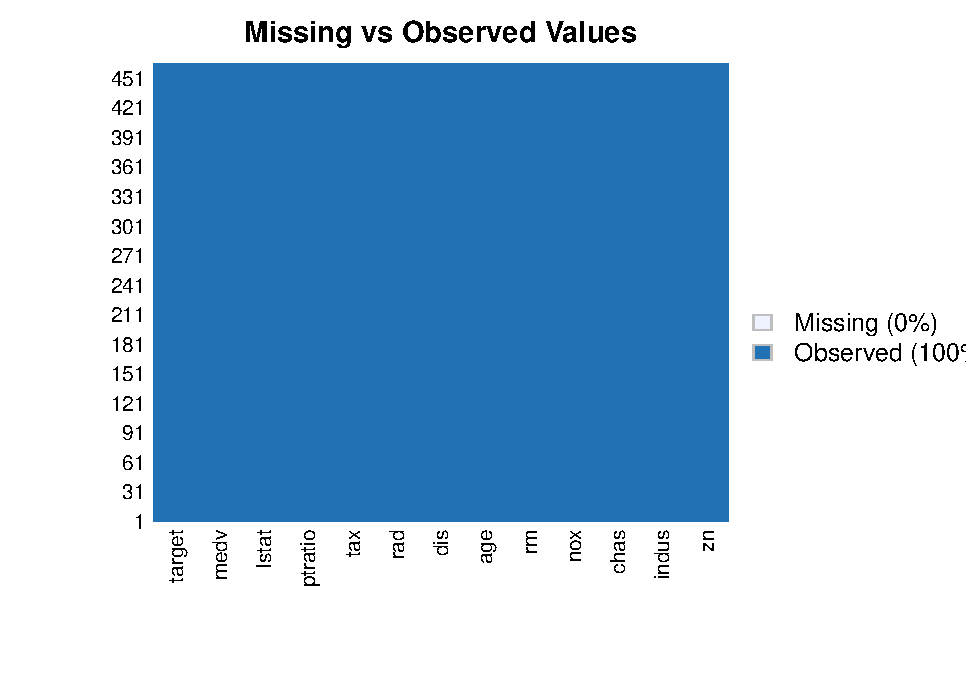
\includegraphics{HW3_files/figure-latex/unnamed-chunk-5-1.pdf}

\begin{Shaded}
\begin{Highlighting}[]
\NormalTok{summary.tbl }\OtherTok{\textless{}{-}} \FunctionTok{summary}\NormalTok{(cdata)}
\NormalTok{summary.tbl }\SpecialCharTok{\%\textgreater{}\%} 
\NormalTok{  kable }\SpecialCharTok{\%\textgreater{}\%} 
  \FunctionTok{kable\_styling}\NormalTok{()}
\end{Highlighting}
\end{Shaded}

\begin{table}[H]
\centering
\begin{tabular}{l|l|l|l|l|l|l|l|l|l|l|l|l|l}
\hline
  &       zn &     indus &      chas &      nox &       rm &      age &      dis &      rad &      tax &    ptratio &     lstat &      medv &     target\\
\hline
 & Min.   :  0.00 & Min.   : 0.460 & Min.   :0.00000 & Min.   :0.3890 & Min.   :3.863 & Min.   :  2.90 & Min.   : 1.130 & Min.   : 1.00 & Min.   :187.0 & Min.   :12.6 & Min.   : 1.730 & Min.   : 5.00 & Min.   :0.0000\\
\hline
 & 1st Qu.:  0.00 & 1st Qu.: 5.145 & 1st Qu.:0.00000 & 1st Qu.:0.4480 & 1st Qu.:5.887 & 1st Qu.: 43.88 & 1st Qu.: 2.101 & 1st Qu.: 4.00 & 1st Qu.:281.0 & 1st Qu.:16.9 & 1st Qu.: 7.043 & 1st Qu.:17.02 & 1st Qu.:0.0000\\
\hline
 & Median :  0.00 & Median : 9.690 & Median :0.00000 & Median :0.5380 & Median :6.210 & Median : 77.15 & Median : 3.191 & Median : 5.00 & Median :334.5 & Median :18.9 & Median :11.350 & Median :21.20 & Median :0.0000\\
\hline
 & Mean   : 11.58 & Mean   :11.105 & Mean   :0.07082 & Mean   :0.5543 & Mean   :6.291 & Mean   : 68.37 & Mean   : 3.796 & Mean   : 9.53 & Mean   :409.5 & Mean   :18.4 & Mean   :12.631 & Mean   :22.59 & Mean   :0.4914\\
\hline
 & 3rd Qu.: 16.25 & 3rd Qu.:18.100 & 3rd Qu.:0.00000 & 3rd Qu.:0.6240 & 3rd Qu.:6.630 & 3rd Qu.: 94.10 & 3rd Qu.: 5.215 & 3rd Qu.:24.00 & 3rd Qu.:666.0 & 3rd Qu.:20.2 & 3rd Qu.:16.930 & 3rd Qu.:25.00 & 3rd Qu.:1.0000\\
\hline
 & Max.   :100.00 & Max.   :27.740 & Max.   :1.00000 & Max.   :0.8710 & Max.   :8.780 & Max.   :100.00 & Max.   :12.127 & Max.   :24.00 & Max.   :711.0 & Max.   :22.0 & Max.   :37.970 & Max.   :50.00 & Max.   :1.0000\\
\hline
\end{tabular}
\end{table}

\begin{Shaded}
\begin{Highlighting}[]
\FunctionTok{set.seed}\NormalTok{(}\DecValTok{72747}\NormalTok{)}
\NormalTok{indecies }\OtherTok{\textless{}{-}} \FunctionTok{createDataPartition}\NormalTok{(cdata}\SpecialCharTok{$}\NormalTok{target, }\AttributeTok{p =}\NormalTok{ .}\DecValTok{7}\NormalTok{, }\AttributeTok{list =} \ConstantTok{FALSE}\NormalTok{, }\AttributeTok{times =} \DecValTok{1}\NormalTok{)}
\NormalTok{train }\OtherTok{\textless{}{-}}\NormalTok{ cdata[indecies,]}
\NormalTok{test }\OtherTok{\textless{}{-}}\NormalTok{ cdata[}\SpecialCharTok{{-}}\NormalTok{indecies,]}
\end{Highlighting}
\end{Shaded}

\begin{Shaded}
\begin{Highlighting}[]
\NormalTok{train }\SpecialCharTok{\%\textgreater{}\%}
  \FunctionTok{select}\NormalTok{(}\SpecialCharTok{{-}}\NormalTok{target) }\SpecialCharTok{\%\textgreater{}\%}
  \FunctionTok{summary}\NormalTok{() }\SpecialCharTok{\%\textgreater{}\%}
  \FunctionTok{kable}\NormalTok{() }\SpecialCharTok{\%\textgreater{}\%}
  \FunctionTok{kable\_styling}\NormalTok{()}
\end{Highlighting}
\end{Shaded}

\begin{table}[H]
\centering
\begin{tabular}{l|l|l|l|l|l|l|l|l|l|l|l|l}
\hline
  &       zn &     indus &      chas &      nox &       rm &      age &      dis &      rad &      tax &    ptratio &     lstat &      medv\\
\hline
 & Min.   :  0.00 & Min.   : 0.46 & Min.   :0.00000 & Min.   :0.3920 & Min.   :3.863 & Min.   :  2.90 & Min.   : 1.174 & Min.   : 1.000 & Min.   :188.0 & Min.   :12.60 & Min.   : 1.92 & Min.   : 5.00\\
\hline
 & 1st Qu.:  0.00 & 1st Qu.: 5.19 & 1st Qu.:0.00000 & 1st Qu.:0.4480 & 1st Qu.:5.878 & 1st Qu.: 43.10 & 1st Qu.: 2.105 & 1st Qu.: 4.000 & 1st Qu.:281.0 & 1st Qu.:16.90 & 1st Qu.: 7.06 & 1st Qu.:16.80\\
\hline
 & Median :  0.00 & Median : 9.69 & Median :0.00000 & Median :0.5380 & Median :6.226 & Median : 77.30 & Median : 3.132 & Median : 5.000 & Median :335.0 & Median :18.90 & Median :11.74 & Median :21.00\\
\hline
 & Mean   : 10.45 & Mean   :11.15 & Mean   :0.06422 & Mean   :0.5536 & Mean   :6.303 & Mean   : 68.44 & Mean   : 3.762 & Mean   : 9.153 & Mean   :406.2 & Mean   :18.38 & Mean   :12.66 & Mean   :22.37\\
\hline
 & 3rd Qu.: 12.50 & 3rd Qu.:18.10 & 3rd Qu.:0.00000 & 3rd Qu.:0.6240 & 3rd Qu.:6.638 & 3rd Qu.: 93.95 & 3rd Qu.: 5.117 & 3rd Qu.: 8.000 & 3rd Qu.:666.0 & 3rd Qu.:20.20 & 3rd Qu.:16.56 & 3rd Qu.:24.80\\
\hline
 & Max.   :100.00 & Max.   :27.74 & Max.   :1.00000 & Max.   :0.8710 & Max.   :8.725 & Max.   :100.00 & Max.   :10.710 & Max.   :24.000 & Max.   :711.0 & Max.   :22.00 & Max.   :36.98 & Max.   :50.00\\
\hline
\end{tabular}
\end{table}

\hypertarget{data-preparation}{%
\subsection{Data Preparation}\label{data-preparation}}

Describe how you have transformed the data by changing the original
variables or creating new variables. If you did transform the data or
create new variables, discuss why you did this. Here are some possible
transformations. a. Fix missing values (maybe with a Mean or Median
value) b. Create flags to suggest if a variable was missing c.~Transform
data by putting it into buckets d.~Mathematical transforms such as log
or square root (or use Box-Cox) e. Combine variables (such as ratios or
adding or multiplying) to create new variables

\hypertarget{build-models}{%
\subsection{Build Models}\label{build-models}}

Using the training data, build at least three different binary logistic
regression models, using different variables (or the same variables with
different transformations). You may select the variables manually, use
an approach such as Forward or Stepwise, use a different approach, or
use a combination of techniques. Describe the techniques you used. If
you manually selected a variable for inclusion into the model or
exclusion into the model, indicate why this was done. Be sure to explain
how you can make inferences from the model, as well as discuss other
relevant model output. Discuss the coefficients in the models, do they
make sense? Are you keeping the model even though it is counter
intuitive? Why? The boss needs to know.

\hypertarget{select-models}{%
\subsection{Select Models}\label{select-models}}

Decide on the criteria for selecting the best binary logistic regression
model. Will you select models with slightly worse performance if it
makes more sense or is more parsimonious? Discuss why you selected your
models. For the binary logistic regression model, will you use a metric
such as log likelihood, AIC, ROC curve, etc.? Using the training data
set, evaluate the binary logistic regression model based on (a)
accuracy, (b) classification error rate, (c) precision, (d) sensitivity,
(e) specificity, (f) F1 score, (g) AUC, and (h) confusion matrix. Make
predictions using the evaluation data set

\hypertarget{conclusion}{%
\subsection{Conclusion}\label{conclusion}}

\end{document}
